\section{Why \& how do people stream creative work?}
%Now that we have a broad understanding of two popular creative livestreaming communities, we seek to go deeper into the motivations and processes behind creative livestreamers. 
What motivates people to livestream creative work? What challenges do they encounter in the process, and how do these compare with streamers in other domains? We interviewed 8 creative livestreamers and found that streamers were primarily motivated by sharing and engaging with their audience. However, they find it difficult to connect with their audience while focusing on their work. Additionally, for many, livestreaming requires significant effort and behind-the-scenes preparation. 

%Streamer motivations and processes seem to be highly dependent on the type of stream they create. Prior work has shown that the main reasons gaming streamers stream are to build a community of like-minded individuals \cite{Hamilton2014, Pellicone2017} and to make money or promote their personal brand \cite{Pellicone2017}. People who livestream about their lifestyle or to entertain do it primarily for personal branding \cite{Tang2016}. In contrast, educational or culture-sharing streamers' main goal is usually to share their knowledge and culture with others \cite{Lu2018a, Lu2019}. As for process, some livestreams are highly produced and require significant preparation beforehand (\textit{e.g.,} e-sports tournaments), while others occur on-the-spot whenever the streamer decides to go live (\textit{e.g.,} many lifestyle streams on Instagram).
%Such streamers often care more about making a broad positive impact and raising awareness about their particular activity than making money or receiving gifts from viewers, even when they do also make money as a side benefit \cite{Lu2019}. 
%We echo Lu et al.'s \cite{Lu2019} finding (maybe) that for many types of creative activities that are usually solitary (e.g., playing a solo musical instrument or doing visual art), streaming allows people to have company while they work so the activity is not so lonely.

\begin{table*}[b]
\centering
\caption{Self-reported background information about the eight creative livestreamers we interviewed. ``Skill'' refers to the streamer's skill at the type of creative work they stream. After interviewing the streamers, we determined the structure type of their most frequent streaming style.}~\label{table:livestream_streamers}
\resizebox{1\textwidth}{!}{
\begin{tabular}{llllllll}
            & \textbf{Role}                                                                       & \textbf{Content}       & \textbf{Skill} & \textbf{Frequency} & \textbf{Platform}                                                              & \textbf{Primary type} & \textbf{Moderators} \\
\textit{P1} & Freelance Digital Illustrator                                                       & Digital Illustration   & Expert         & 3 times / week     & Twitch                                                                         & Making                & Yes        \\
\textit{P2} & \begin{tabular}[t]{@{}l@{}}Video Editor \& Educational\\ Content Maker\end{tabular} & Q\&A, Analyzing Videos & Expert         & Occasional         & YouTube, Instagram                                                             & Teaching              & Yes        \\
\textit{P3} & Artist / Musician                                                                   & Music Improvisation    & Expert         & Occasional         & Facebook, Instagram                                                            & Performing            & No         \\
\textit{P4} & Drawing Hobbyist                                                                    & Digital Drawing        & Intermediate   & Monthly            & Twitch                                                                         & Making                & No         \\
\textit{P5} & Drawing Hobbyist                                                                    & Digital Drawing        & Intermediate   & Monthly            & Twitch, previously Picarto                                                     & Making                & No         \\
\textit{P6} & Adobe XD Evangelist                                                                 & UX Design              & Expert         & Daily - Weekly     & \begin{tabular}[t]{@{}l@{}}YouTube, Facebook,\\ previously Twitch\end{tabular} & Teaching/Making       & Yes        \\
\textit{P7} & Adobe XD Evangelist                                                                 & UX \& Graphic Design   & Expert         & 3 times / week     & \begin{tabular}[t]{@{}l@{}}YouTube, Periscope,\\ Facebook\end{tabular}         & Teaching/Making       & Yes        \\
\textit{P8} & Adobe Designer                                                                      & UX \& Graphic Design   & Expert         & Daily - Weekly     & YouTube, previously Twitch                                                     & Teaching/Making       & Yes       
\end{tabular}
}
\end{table*}



\subsection{Interview methodology}
We recruited 8 streamers (4 male, 4 female, ages 20-45) from personal and professional connections for one-hour semi-structured interviews. We interviewed people across creative disciplines and experience with streaming (\autoref{table:livestream_streamers}). We asked participants about their current position and background, process and motivation for streaming, challenges and successes they have experienced, and strategies for engaging with their audience. Three of the participants also host for \textit{Adobe Live}; we asked them about their experience hosting as well as streaming. We took notes and recorded every interview, and analyzed them by comparing participants' answers and identifying common patterns. Interviews were conducted over video chat (4), audio chat (2), or in person (2). Each participant received a \$15 gift card for their time. 


\subsection{About the streamers}

\textit{P1} is a freelance artist who began streaming her work full-time on Twitch in 2016. For the first two years, she streamed for 20-25 hours a week and spent the rest of her time on stream-related preparation. At this commitment level, streaming was her primary source of income. Income on platforms like Twitch mainly derives from ad revenue, viewer subscriptions, and donations. Over time, this became exhausting and felt unsustainable. \textit{P1} took a break, and now streams casually 3 times a week but not as a primary source of income. Her livestream setup includes a camera view of her face, a screencast of her work, a Stream Deck (\autoref{fig:livestream_streamdeck}), and two monitors for her to see chat activity and other information.

\begin{figure}[b]
\centering
  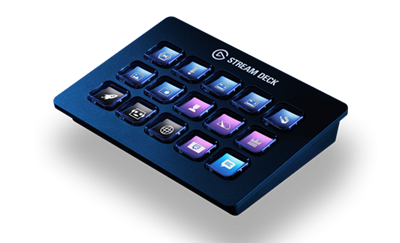
\includegraphics[width=0.6\columnwidth]{livestreams/figures/streamdeck.png}
  \caption{The Stream Deck is a programmable control pad used by many streamers, including \textit{P1}, for easy access to common shortcuts and actions. It integrates with Open Broadcaster Software (OBS), a program used by many streamers to host their livestreams (\href{https://www.elgato.com/en/gaming/stream-deck}{\nolinkurl{elgato.com/en/gaming/stream-deck}}).}~\label{fig:livestream_streamdeck}
  \vspace{-0.2in}
\end{figure}

\textit{P2} is a video editor and creator who has been making video tutorials on photo and video editing for about 7 years. He hosts a podcast where he interviews people about their creative approach and life stories. He has tried Periscope, and began streaming on YouTube when it enabled mobile streaming in 2017: casual streaming was on the rise. Occasionally he livestreams on YouTube or Instagram, answering viewer questions, teaching a particular topic, analyzing a popular video, or critiquing viewers' work. His setup comprises a camera view of his face, a screencast of his work, and a large monitor for him to see chat activity and other information.

\textit{P3} is a musician who livestreams on Facebook and Instagram (with three band members). Her streams are spontaneous and improvisational; the quartet does not play together regularly but they have a fan base that they stream to whenever they are together. These livestreams require little setup; they are broadcast from a single mobile phone either held by a friend or propped up. She also occasionally livestreams product reviews and behind-the-scenes views of her shows.

\textit{P4} and \textit{P5} are hobby artists who stream digital drawing about once a month on Twitch. They both started livestreaming 2 or 3 years ago. \textit{P5} used to stream on Picarto, and moved to Twitch about a month ago because it was easier to use and tends to attract more viewers as a better-known platform. \textit{P5} rarely talks out loud during her streams (only when nobody else is home) and \textit{P4} never does. Instead, they engage with viewers by typing in the chat. Neither shows their face when streaming; their setups include only a screencast of their drawing window. 

\textit{P6}, \textit{P7}, and \textit{P8} stream as part of their jobs at Adobe by hosting artists, streaming their own work, and teaching Adobe products.
%are all employees of Adobe who regularly stream on Adobe's Daily Creative Challenges, and also host on Adobe Live. 
%These participants stream frequently as part of their jobs, and are all highly experienced at the creative work they stream. 
\textit{P6} has been making video tutorials on photo editing for over 10 years. He briefly tried streaming on Twitch but found that his audience did not transfer over to the new platform. He has been streaming with Adobe for approximately 6 months. \textit{P7} taught courses and training programs on design and illustration software for many years. He has been working at Adobe for 9 years, and streaming with Adobe for about 4 years. 
%\textit{P7} was one of the first evangelists involved in Adobe's livestreaming efforts, which started on Twitch.
\textit{P8} is a designer and trained illustrator and has been streaming with Adobe for 4 years. Before joining Adobe, she used to occasionally stream her art process on Twitch. By virtue of livestreaming professionally, all three participants have fairly sophisticated technology setups, including a camera view of their face in front of a green screen, a screencast of their computer, several displays for them to see chat activity and other information, and sometimes additional cameras (\autoref{fig:livestream_adobelive_setup}). 

\begin{figure}[t]
\centering
  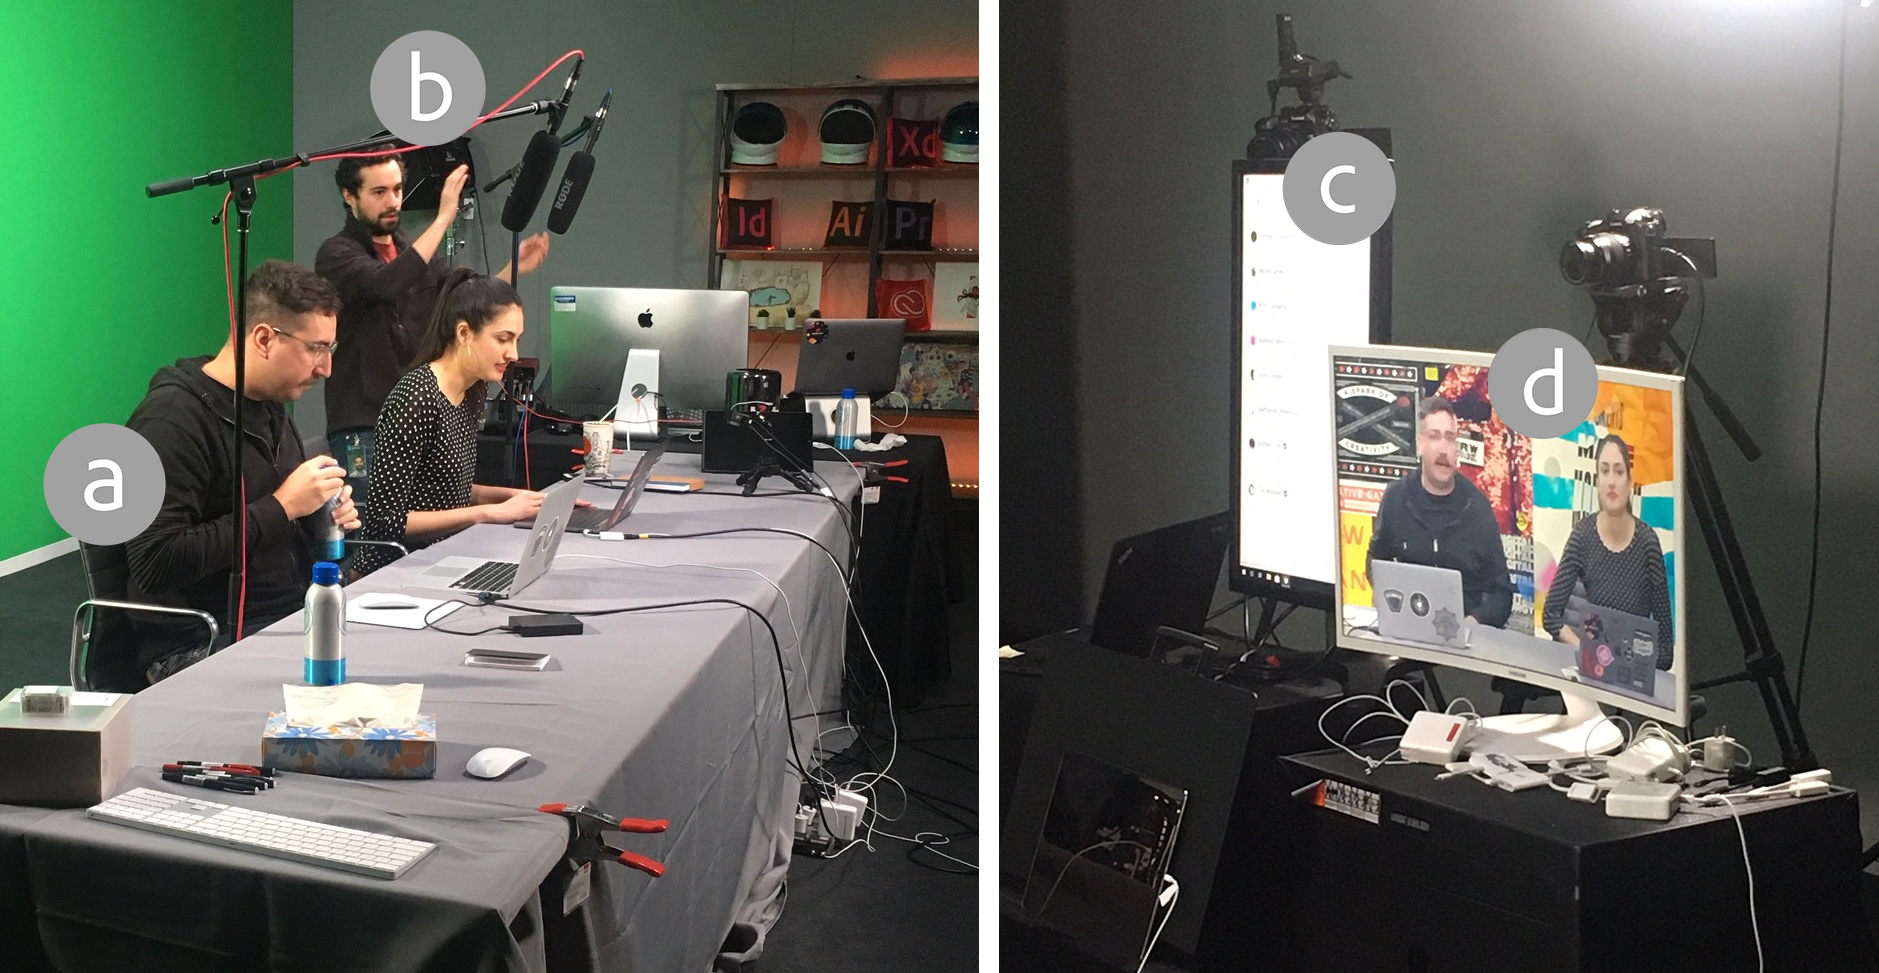
\includegraphics[width=1\columnwidth]{livestreams/figures/adobelive_setup.png}
  \caption{The technical setup for \textit{Adobe Live}. (a) The artist (left) and host (right) sit in front of a green screen, with both computers connected for screencasting. (b) Behind the scenes, at least one person helps with technical support, including setup, testing, and monitoring. (c) The artist and host see a display with the live chat feed, and (d) a display showing how they currently appear in the livestream. }~\label{fig:livestream_adobelive_setup}
  \vspace{-0.2in}
\end{figure}

\subsection{Findings}
\subsubsection{Audience engagement is a primary goal for streamers}
Like with gaming \cite{Pellicone2017, Hamilton2014} and culture-sharing \cite{Lu2019} livestreams, audience engagement is important to creative streamers. All participants said they engage with their audience during streams, despite their different personalities and streaming styles. When asked about their main motivation for livestreaming, participants mentioned creating a space for people to hang out together, building an audience, sharing their process with others, and engaging in meaningful conversations.

When asked for an example of a rewarding or enjoyable moment, every participant mentioned audience engagement in some way. Three participants mentioned feeling rewarded by gratitude from viewers for inspiration and community. This inspiration goes both ways: \textit{P5} mentioned that she has received valuable feedback from a viewer that helped improve her own work. Two participants valued that \textit{``there's something more authentic about [livestreaming] ... it allows me to just be myself more authentically and people can pick up on that, they can understand what you're really about in a way that you just can't express via [other modalities]''} (\textit{P2}). \textit{``There are really no mistakes, there's just honesty''} (\textit{P3}).

A key difference between gaming and creative livestreams affecting engagement is the scale of the audience. The average live audience size for our participants ranged from about 5 to 1000, with most sitting at the lower end. Popular streamers of video games such as Fortnite or League of Legends often average audiences of between 2000 and 40,000. This means that creative streamers often feel a tighter personal connection with their viewers, while viewers of gaming streams tend to mostly interact with each other, as the chat goes too quickly for the streamer to keep up \cite{Lessel2017, Hu2017}.

\textit{P7} expressed a desire to offer the audience more diverse interactive experiences beyond just text chat. Currently, gaming livestreams sometimes host ``audience participation games'' \cite{Glickman2018}. \textit{P1} often organizes games during livestreams, such as contests with prizes, voting on what she should do next, or ``prompt games'' where viewers contribute ideas. \textit{P4} did a ``request stream'', where he drew whatever viewers requested, and \textit{P2} often runs Q\&A-form streams, where he will open an application and just let the audience ask questions. As he put it, \textit{``I want to do what they want to do.''} \textit{Adobe Live} often has giveaways for audience participation, and Adobe hosts a \textit{Daily Creative Challenge}. This kind of engagement \textit{``make[s] it a collaborative thing''} (\textit{P6}), increasing audience investment.

One emerging practice is livestreaming portfolio critiques. Like a call-in radio show or newspaper advice column, a few people get direct feedback, and many people benefit through over-the-shoulder learning. This form of learning can be extremely beneficial \cite{Lopez2010}; it is notable that there is a streaming audience that seeks it out. Similar to shows and columns, streamers have the challenge of selecting which submission(s) to critique. \textit{P2} initially handled this with chat but was quickly overwhelmed by the number of messages. To address this, he found and installed a widget\footnote{\href{https://streamlabs.com/widgets}{\nolinkurl{streamlabs.com/widgets}}} to help him select submissions and allow users to pay a small amount to have their work critiqued. While valuable, it takes time and effort to manage such tools. This also exacerbates streaming's already ``fragmented technology ecosystem'' \cite{Lu2019}.

Aside from the three Adobe participants who stream as part of their jobs, none of the participants currently stream as a major income source. Though these participants were not \textit{primarily} motivated by monetary gain, two mentioned that it was a significant secondary benefit, \textit{e.g., } \textit{P4} said, \textit{``it doesn't matter how good my work gets if I don't actually market myself.''} Many streamers in other domains (especially video games) also aim to grow their audience and make money \cite{Pellicone2017}. \textit{P1}'s sought to eventually be a self-sustaining artist; she emphasized that her primary goal was building the audience and creating a positive community; \textit{``I believe that the audience brings [financial benefits].''} \textit{P3} wished it was easier for viewers to donate. Compensation is possible on some platforms (\textit{e.g.,} Twitch) but requires configuration.

\subsubsection{Moderators \& hosts alleviate common challenges for artists}
A big part of engaging with the audience is interacting via the chat window with viewers' questions, comments, and feedback. 
%interesting: this is indirect engagement
Most participants said they sometimes have trouble keeping up with the chat as it requires switching focus from their creative work. This split-attention challenge echoes previous findings for programming \cite{Faas2018} and culture-sharing \cite{Lu2019} streams.
%- Paying attention to chat and interacting with audience while working \cite{Faas2018}, especially when work is not on the computer \cite{Lu2019} \\
%-- Messages distracting from work, especially when lots of viewers \cite{Lu2019}
\textit{P5} even said, \textit{``I usually put a warning beforehand that I'm not the most talkative while I'm drawing but I try to check up on the chat as often as I can.''} For \textit{P3} who streams on  a smartphone, it is even harder to pay attention to chat, as it requires stopping her performance and coming up close to the camera.

Moderators are one way to alleviate this challenge for viewers. In large gaming livestreams, trolling is common; many streamers have dedicated moderators whose main role is to ban or time-out people posting inappropriate content and enforce a streamer's community guidelines \cite{Seering2017, Lo2018, Seering2019, YvetteWohn2019}. Trolls are seen less often in smaller livestreams, yet still appear; 5/8 participants have dedicated moderators. As prior work has shown  \cite{Lo2018, Seering2019, YvetteWohn2019}, employing successful moderators requires significant preparation; streamers must work with moderators to develop guidelines, and they must constantly work to make sure their judgments align. \textit{P1} and \textit{P2} echoed these challenges: \textit{P1} has spent significant time making a document of guidelines for her moderators. \textit{P2} has not, and as a result finds that their judgments do not always align: \textit{``They might want to ban someone that I think is fine, or they might not ban someone that I think should be banned.''}

While moderators can help enforce basic rules and keep the chat constructive, they usually do not support streamers' \textit{engagement} with their audience. Viewers often have questions, feedback, and suggestions for the streamer; these are easily missed. Some moderators do engage in the chat \cite{YvetteWohn2019} but they require training in order to answer questions on behalf of the streamer (\textit{e.g.,} \textit{P1}'s moderators). In addition, some streamers find it difficult to talk out loud to their viewers: both \textit{P4} and \textit{P5} said they would like to have others to talk with, as they did not want to fill the silence alone; \textit{``I'm mostly intimidated by the idea of me having to fill a lot of void space''} (\textit{P4}). While \textit{P4} used Discord and \textit{P5} sometimes used join.me for voice chat, these require extra work on the part of the streamer, and sit outside of the main livestream platform.

A different facilitation role that Adobe streams employ to address these challenges are \textit{hosts}. \textit{Adobe Live} streams feature paid hosts who keep the artist and audience engaged, help artists feel confident, and help them focus on their work. The host watches chat messages come in, says hi and responds out loud to viewers' messages, and decides which of viewers' questions to ask to the artist. As \textit{P7} put it, the host is the \textit{``representative for the chat.''} Hosts strive to keep viewers engaged by asking the chat questions and including viewers' names when they respond to them. Hosts also strive to keep the \textit{artist} engaged and talking. As \textit{P6} put it, \textit{``the last thing you want is dead silence.''} This can be difficult when the artist is shy or quiet, so hosts have picked up tricks such as asking the artist questions about themselves, choosing questions from the chat that are likely to start a conversation, and switching the feed briefly over to their computer to show a relevant tip or trick.


%xxx: commenting out for now
%- moderators can be co-present or telepresent
%- some streamers sometimes have co-present people (helping, audience, etc)

\subsubsection{Different platforms bring different audiences}
Some participants stream on multiple platforms. Some start streaming on one platform and then switch to another. This brought up interesting trade-offs between different types of livestreaming platforms. Besides mobile platforms being simpler than desktop, different platforms also bring different audiences. \textit{P6} and \textit{P8} used to stream on Twitch before Adobe's livestreaming community started. They explained that Twitch is a general-purpose platform dedicated to livestreaming. It attracts people who generally enjoy livestreams and may be interested in creative work but are less often professional. On Twitch it's harder to attract people who are less familiar with livestreams, perhaps because of unique specific features such as ``emotes''; as \textit{P1} explained, \textit{``if you are in the ecosystem you're really happy with it, and if you're not in the ecosystem it's bizarre.''}

\textit{Adobe Live} is an example of a professionally-managed live\-stream aimed at a company's customers. As a result, it tends to attract aspiring designers and creatives who use the software being shown and want to learn how to produce better work. It also attracts more people who are not familiar with livestreaming, as it is shown on platforms that also include other forms of media (Behance and YouTube). A challenge with platforms like this is that \textit{``people might not really get ... why watch a livestream''} (\textit{P2}), as it is not yet widely understood.

Finally, platforms like Picarto focus specifically on \textit{creative} livestreaming. These attract viewers dedicated to the topic, which can make conversations more focused. The challenge with specific platforms like these (at least in an era where the phenomenon is still growing) is that fewer people have heard of them, so it can be harder to attract viewers. For this reason, \textit{P5} switched to Twitch. Indeed, Picarto generally has 100-200 streams live at any given time, which is considerably less than the Art section alone on Twitch (which has over 300).

The type of creative work being done also affects the audience. For participants who do visual art such as drawing or use creative software, their streams tend to be of the Making or Teaching type, and their audiences mainly comprise other artists or people interested in learning the skill. For \textit{P3} who streams Performing content on Facebook, her audience mainly consists of friends and fans. These viewers enjoy watching the performance and being a part of live music, but are not necessarily looking to learn music themselves.
 
%\subsection{Streaming often requires setup and preparation}
\subsubsection{Amount of preparation depends on stream type \& preferences}
While gaming livestreamers can simply turn on their screencast and begin playing a game, creative streaming often requires more preparation. 6/8 participants said they prepare before beginning a livestream. Four of these primarily run Teaching streams; the other two primarily run Making streams. For Teaching streams (\textit{P2}, \textit{P6}, \textit{P7}, and \textit{P8}), the streamers spend time before the stream going over what they will show. For Making streams, \textit{P1} and \textit{P5} spend time on the early stages of their creative work. In addition to preparing content, livestreaming (especially on desktop platforms) also requires technical setup. Most participants who stream on desktop platforms said this takes time: setting up cameras and microphones, organizing windows across multiple displays, and testing the output.

Most Teaching streams require some content preparation, much like how course instructors make lesson plans. Socializing streams likely require little-to-no preparation, as the content of these streams is mainly driven by conversation with viewers. For example, \textit{P2} sometimes streams casual Q\&A streams on Instagram, enjoying their spontaneous nature: \textit{``you just go live.''} For Making and Performing, preparation time depends on the streamer. Some streamers also announce beforehand when they will stream so that viewers can plan to tune in.
%i said it better. but dont remember how
For casual Performing streams like \textit{P3}'s, all she has to do is turn on the camera and position it. But rehearsed performances require practice beforehand. \textit{P4} said he typically only plans his Making streams 5 minutes before starting, and will start drawing from scratch on the stream. \textit{P8}, who used to do more Making streams, also did not prepare: \textit{``it's as if I am opening up my sketchbook and my friends are there.''} Other Making streamers like \textit{P1} and \textit{P5} prefer to start their work before beginning a stream.

Several participants emphasized that some activities make for more engaging livestreams than others. Both \textit{P1} and \textit{P5} said their streams are most successful when they do initial sketching beforehand, then spend the stream filling it in and coloring. This is because the early ideation stages involve more problem-solving and deep thinking: \textit{``to be able to put that full energy ... to get through the failures and to find the successes -- I can't multitask it.''} \textit{P5} also felt this early stage was less appealing for audiences: \textit{``For a long while they're going to have to look at a blank sheet of white `paper' so they don't really see the sketches right away ... I think that loses their attention.''} \textit{P2}, when asked why he doesn't livestream his video editing process, he said he tried it but it was too difficult to focus: \textit{``when you're video editing you need to listen to music and focus ... when you're streaming you need to be engaging with the chat.''} This echoes previous findings for knowledge-sharing \cite{Lu2018a} and programming \cite{Faas2018} streams; streamers often prepare beforehand to ensure that the content being streamed will be entertaining for viewers and will not require too much focus on the streamer's part. 

% other challenges:
% -- Delay between video and chat \cite{Lessel2017} \\
% - Entertaining both novice and expert viewers \cite{Faas2018}
% - fragmented technology ecosystem, hard to manage everything \cite{Lu2019}
% - narrating while also focusing on work \cite{Faas2018} \\
% -- Balancing entertainment with showing realistic process \cite{Faas2018} \\

\subsubsection{Permanence of livestream archives affects performance}
We found that the ability to archive livestreams significantly affects how streamers perform. Several interviewees mentioned that attentiveness to viewers of a future recording influenced their choices in the moment. \textit{P7} said he sometimes records learning-focused livestreams that are meant to be useful as replays, and he interacts less with viewers during those streams. \textit{P2} often deletes or hides his completed livestreams because they look less polished than his regular tutorial videos. 
\textit{P4} and \textit{P5} don't archive their videos, as \textit{``[livestreaming is] more of a in-the-moment [thing]''} (\textit{P5}). 